\documentclass{article}

\usepackage{graphicx}
\pagestyle{plain}
\usepackage[utf8]{inputenc}
\usepackage[T1]{fontenc}
\usepackage{polish}

\author{Patryk Jędrzejko 200406}
\title{Sprawozdanie z laboratorium - PAiMSI.}
\begin{document}
\maketitle

\section{Wprowadzenie}
W danym ćwiczeniu należało napisać program, który zapełniałby strukturę stosu bądź też kolejki
za pomocą tablicy lub listy.
\\Program porównuję wypełnianie następujących struktur:
\\- stos za pomocą tablicy
\\- stos za pomocą listy
\\- kolejki za pomocą tablicy
\\- kolejki za pomocą listy
\\
\\Dane do zapełniania poszczególnych struktur są umieszczone w plikach pod nazwami: stos.txt, stos100.txt,
stos1000.txt oraz stos10000.txt. Gdzie każdy kolejny plik zawiera więcej danych, tzn. od 10
elementów do 10000 elementów. W każdym pliku pierwsza wartość to liczba elementów w danym pliku.

\section{Tabela wyników oraz wykres}
\\ W sprawozdaniu zamieszczony jest wykres przedstawiający zależność
czasu od ilości elementów oraz tabela wyników tej zależności.
\subsection{Tabela wyników}
Tabela wyników - znajduję się na stronie nr 3.
\begin{figure}[H]
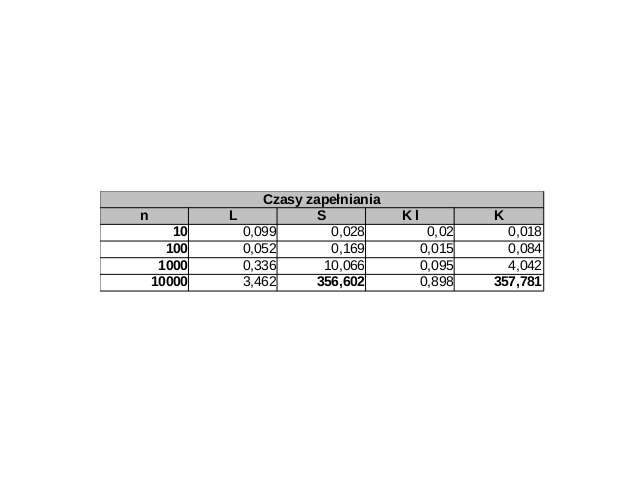
\includegraphics[width=\textwidth]{tabela.png}
\caption{Tabela wyników zapełniania.}
\label{fig:tabela.png}
\end{figure}
\subsection{Wykres}
Wykres przedstawiający czas zapełnienia od ilości elementów w pliku - znajduję się na stronie nr 4.
\begin{figure}[H]
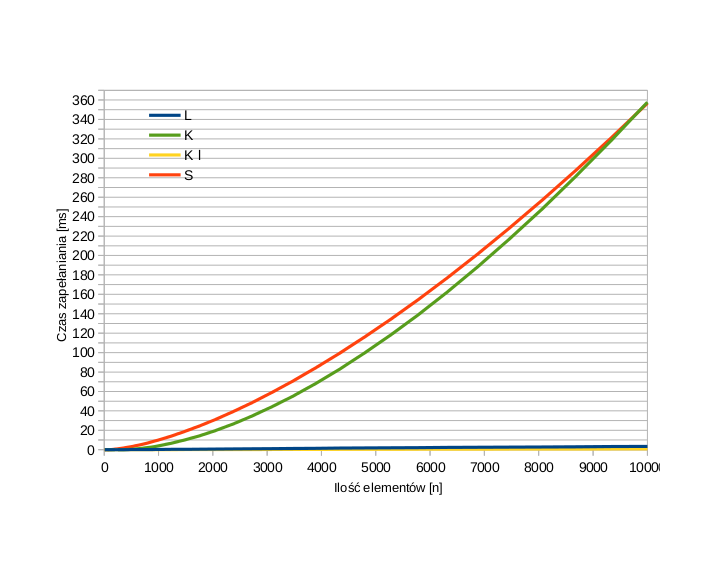
\includegraphics[width=\textwidth]{wykres.png}
\caption{Wykres przedstawiąjący czas zapełnienia od ilości elementów.}
\label{fig:wykres.png}
\end{figure}


\section{Wnioski:}
\begin{itemize}
\item Patrząc na wyniki zapełniania struktur widzimy, iż najszybciej zapełnianie wykonuje
się dla struktury kolejki za pomocą listy. Dlatego można stwierdzić, że ten sposób implementacji
struktury zapełniającej jest najszybszą implementacją dla tych struktur.
\item Niestety dwa wyniki dla n = 10000 elementów, dla stosu za pomocą tablicy oraz kolejki za pomocą tablicy odbiegają od reszty struktur. Jest to wywołane błędem w programie, którego niestety nie udało mi 
się naprawić. Błąd występuje dopiero dla n = 10000 elementów.
\item Na koniec można stwierdzić, iż struktura kolejki okazała się szybsza niż struktura stosu.

\end{itemize}
\\
Wykresy oraz tabela wyników znajduję się również osobno w katalogu programu (wykres.pdf, tabela wynikow.pdf).

\end{document}
